% !TeX program = xelatex
% 完整主文件；XeLaTeX编译两遍。图片放在images目录，Logo保留brand目录；数值图表为TikZ或原生表格。
\documentclass[aspectratio=169,compress,11pt]{beamer}
\usetheme{Singapore}
\usepackage[UTF8,fontset=fandol]{ctex}
\usepackage{amsmath,booktabs,tabularx,array,tikz,graphicx}
\usefonttheme[onlymath]{serif}
\setlength{\abovedisplayskip}{0.45em}
\setlength{\belowdisplayskip}{0.4em}
\setCJKsansfont{FandolSong-Regular.otf}[BoldFont=FandolSong-Bold.otf]
\usetikzlibrary{positioning,arrows.meta}
\definecolor{lightblue}{RGB}{45,45,235}
\definecolor{navgray}{RGB}{137,141,177}
\definecolor{scured}{RGB}{154,25,42}
\setbeamercolor{structure}{fg=lightblue}
\setbeamercolor{frametitle}{fg=lightblue}
\setbeamerfont{frametitle}{size=\Large,series=\mdseries}
\setbeamercolor{title}{fg=lightblue}
\setbeamertemplate{frametitle}[default][center]
\addtobeamertemplate{frametitle}{\vspace{-0.12cm}}{}
\setbeamertemplate{navigation symbols}{}
\setbeamertemplate{blocks}[rounded][shadow=false]
\setbeamercolor{block title}{bg=scured!90!black,fg=white}
\setbeamercolor{block body}{bg=scured!6,fg=black}
\setbeamercolor{block title example}{bg=teal!65!black,fg=white}
\setbeamercolor{block body example}{bg=teal!5,fg=black}
\setbeamercolor{block title alerted}{bg=orange!85!black,fg=white}
\setbeamercolor{block body alerted}{bg=orange!7,fg=black}
\setbeamerfont{block title}{size=\normalsize}
\setbeamerfont{block body}{size=\small}
\setbeamertemplate{itemize item}[triangle]
\setbeamertemplate{itemize subitem}[circle]
\setlength{\parindent}{0pt}
\setlength{\parskip}{0.15em}
\setbeamersize{text margin left=0.75cm,text margin right=0.75cm}
\setbeamercolor{author in head/foot}{bg=blue!20,fg=black}
\setbeamercolor{title in head/foot}{bg=blue!16,fg=black}
\setbeamercolor{date in head/foot}{bg=blue!20,fg=black}
\IfFileExists{brand/qi-wang-logo.pdf}{\def\qwlogofile{brand/qi-wang-logo.pdf}}{\def\qwlogofile{../brand/qi-wang-logo.pdf}}
\newcommand{\qwcoverlogo}{\begin{tikzpicture}[remember picture,overlay]\node[anchor=north,inner sep=0pt] at ([yshift=-6.8cm]current page.north){\includegraphics[width=3.7cm]{\qwlogofile}};\end{tikzpicture}}
\newcommand{\currentweeklabel}{导入}
\setbeamertemplate{footline}{\leavevmode\hbox{\begin{beamercolorbox}[wd=.33\paperwidth,ht=2.5ex,dp=1ex,center]{author in head/foot}\raisebox{-0.6pt}{\includegraphics[height=0.27cm]{\qwlogofile}}\hspace{0.7em}\scriptsize 王奇（四川大学）\end{beamercolorbox}\begin{beamercolorbox}[wd=.34\paperwidth,ht=2.5ex,dp=1ex,center]{title in head/foot}\scriptsize 国际金融 · 示范教学\end{beamercolorbox}\begin{beamercolorbox}[wd=.33\paperwidth,ht=2.5ex,dp=1ex,center]{date in head/foot}\scriptsize\currentweeklabel\quad\insertframenumber{} / \inserttotalframenumber\end{beamercolorbox}}}
\setbeamertemplate{headline}{\leavevmode\pgfmathsetmacro{\navwidth}{\paperwidth/1pt}\begin{tikzpicture}[x=1pt,y=-1pt]\path[use as bounding box](0,0)rectangle(\navwidth,20);\shade[top color=blue!8,bottom color=white](0,0)rectangle(\navwidth,20);\ifnum\insertframenumber<1\def\navcol{navgray}\else\ifnum\insertframenumber>5\def\navcol{navgray}\else\def\navcol{lightblue}\fi\fi\node[font=\fontsize{8}{9}\selectfont,text=\navcol] at (40,8) {\hyperlink{slide1}{导入}};\ifnum\insertframenumber<6\def\navcol{navgray}\else\ifnum\insertframenumber>7\def\navcol{navgray}\else\def\navcol{lightblue}\fi\fi\node[font=\fontsize{8}{9}\selectfont,text=\navcol] at (115,8) {\hyperlink{slide6}{识险}};\ifnum\insertframenumber<8\def\navcol{navgray}\else\ifnum\insertframenumber>9\def\navcol{navgray}\else\def\navcol{lightblue}\fi\fi\node[font=\fontsize{8}{9}\selectfont,text=\navcol] at (190,8) {\hyperlink{slide8}{计量}};\ifnum\insertframenumber<10\def\navcol{navgray}\else\ifnum\insertframenumber>15\def\navcol{navgray}\else\def\navcol{lightblue}\fi\fi\node[font=\fontsize{8}{9}\selectfont,text=\navcol] at (265,8) {\hyperlink{slide10}{对冲}};\ifnum\insertframenumber<16\def\navcol{navgray}\else\ifnum\insertframenumber>22\def\navcol{navgray}\else\def\navcol{lightblue}\fi\fi\node[font=\fontsize{8}{9}\selectfont,text=\navcol] at (340,8) {\hyperlink{slide16}{决策}};\ifnum\insertframenumber<23\def\navcol{navgray}\else\ifnum\insertframenumber>26\def\navcol{navgray}\else\def\navcol{lightblue}\fi\fi\node[font=\fontsize{8}{9}\selectfont,text=\navcol] at (415,8) {\hyperlink{slide23}{归纳}};\end{tikzpicture}}\hypersetup{pdftitle={国际金融 · 示范教学},pdfauthor={王奇}}\begin{document}
\renewcommand{\currentweeklabel}{导入}\begin{frame}[t]{}\relax\hypertarget{slide1}{}\fontsize{10.5}{12.8}\selectfont\setlength{\abovedisplayskip}{.25em}\setlength{\belowdisplayskip}{.25em}\begin{tikzpicture}[remember picture,overlay]
\node[anchor=north,font=\fontsize{23}{28}\selectfont,text=lightblue] at ([yshift=-1.55cm]current page.north){外汇风险识别与管理};
\node[anchor=north,align=center,font=\fontsize{13}{19}\selectfont,text=lightblue] at ([yshift=-2.55cm]current page.north){稳健经营，服务实体\\西部外贸企业的风险管理决策};
\node[anchor=north,font=\large] at ([yshift=-4.05cm]current page.north){王奇};
\node[anchor=north] at ([yshift=-4.70cm]current page.north){四川大学商学院};
\node[anchor=north,font=\small] at ([yshift=-5.45cm]current page.north){qiwangphd@scu.edu.cn};
\node[anchor=north] at ([yshift=-6.55cm]current page.north){\includegraphics[width=3.7cm]{\qwlogofile}};
\end{tikzpicture}\note{90分钟两学时；课间休息另计。主课件不含单选题，课堂使用独立配套题目课件。}\end{frame}
\renewcommand{\currentweeklabel}{导入}\begin{frame}[t]{从一笔订单到一项管理决策}\relax\hypertarget{slide2}{}\fontsize{10.5}{12.8}\selectfont\setlength{\abovedisplayskip}{.25em}\setlength{\belowdisplayskip}{.25em}{\fontsize{9.8}{12}\selectfont\renewcommand{\arraystretch}{1.28}\begin{tabularx}{\linewidth}{@{}>{\raggedright\arraybackslash}X>{\raggedright\arraybackslash}X>{\raggedright\arraybackslash}X@{}}\toprule \textbf{企业任务} & \textbf{学习任务} & \textbf{可提交证据}\\\midrule 按期履约，保持预算可预期 & 识别美元净敞口与风险对象 & 合同核对清单\\
在不确定性中选择管理安排 & 比较情景，不依赖单点预测 & 方案计算表与决策单\\
使用AI但不放弃专业责任 & 先算、再核验、再修正 & AI核验记录\\\bottomrule\end{tabularx}}\begin{exampleblock}{本讲目标}给出有计算、有依据、有风险边界的汇率风险管理建议。\end{exampleblock}\end{frame}
\renewcommand{\currentweeklabel}{导入}\begin{frame}[t]{把回信要求落实为专业学习任务}\relax\hypertarget{slide3}{}\fontsize{10.5}{12.8}\selectfont\setlength{\abovedisplayskip}{.25em}\setlength{\belowdisplayskip}{.25em}{\fontsize{9.8}{12}\selectfont\renewcommand{\arraystretch}{1.28}\begin{tabularx}{\linewidth}{@{}>{\raggedright\arraybackslash}X>{\raggedright\arraybackslash}X>{\raggedright\arraybackslash}X@{}}\toprule \textbf{育人联系} & \textbf{本讲的专业任务} & \textbf{观察学生的行动}\\\midrule 服务西部发展与实体经济 & 以西部外贸企业的订单履约为场景 & 说明稳健经营与合同履约的联系\\
交叉融合 & 结合经济分析、财务计算与数字工具 & 用独立计算核验AI建议\\
诚信、敬业与责任 & 如实列出假设、证据及不能保证的结果 & 不隐藏不利情景，不编造运行记录\\\bottomrule\end{tabularx}}\begin{exampleblock}{来源与落实}依据2026年9月28日给四川大学全体师生的回信；将价值要求贯穿案例、活动与评价。\end{exampleblock}\end{frame}
\renewcommand{\currentweeklabel}{导入}\begin{frame}[t]{案例合同与收付款时间线}\relax\hypertarget{slide4}{}\fontsize{10.5}{12.8}\selectfont\setlength{\abovedisplayskip}{.25em}\setlength{\belowdisplayskip}{.25em}\begin{center}
\includegraphics[width=.97\linewidth,height=4.5cm,keepaspectratio,trim=0 0 0 150bp,clip]{figures/01_订单时间线.png}\end{center}{\fontsize{9}{11}\selectfont 企业与数据为课堂案例设定，不对应真实企业经营记录。\par}\begin{exampleblock}{共同参数}三个月后同日：收100万美元，付60万美元；远期结汇\(7.10\,\text{元/美元}\)。\end{exampleblock}\end{frame}
\renewcommand{\currentweeklabel}{导入}\begin{frame}[t]{先读单位，再判断汇率方向}\relax\hypertarget{slide5}{}\fontsize{10.5}{12.8}\selectfont\setlength{\abovedisplayskip}{.25em}\setlength{\belowdisplayskip}{.25em}\begin{columns}[T,onlytextwidth]\begin{column}{.48\textwidth}\begin{itemize}\setlength{\itemsep}{.45em}\item 报价采用\(\frac{\text{元人民币}}{\text{美元}}\)。
\item 7.10降至6.80：每美元换得的人民币减少，人民币升值。
\item 美元净应收不变时，其人民币折算收入下降。\end{itemize}\end{column}\begin{column}{.48\textwidth}{\fontsize{9.8}{12}\selectfont\renewcommand{\arraystretch}{1.28}\begin{tabularx}{\linewidth}{@{}>{\raggedright\arraybackslash}X>{\raggedright\arraybackslash}X@{}}\toprule \textbf{美元净应收40万} & \textbf{人民币金额}\\\midrule 按7.10折算 & 284万元\\
按6.80折算 & 272万元\\
折算金额变化 & 减少12万元\\\bottomrule\end{tabularx}}\end{column}\end{columns}\begin{exampleblock}{注意对象}美元合同金额不因汇率变化自动改变；净收入不等于企业利润。\end{exampleblock}\note{使用独立题目课件Q1、Q2回顾课前诊断。}\end{frame}
\renewcommand{\currentweeklabel}{识险}\begin{frame}[t]{三类外汇风险：对象与时间范围}\relax\hypertarget{slide6}{}\fontsize{10.5}{12.8}\selectfont\setlength{\abovedisplayskip}{.25em}\setlength{\belowdisplayskip}{.25em}\begin{center}
\includegraphics[width=.97\linewidth,height=4.75cm,keepaspectratio,trim=0 0 0 150bp,clip]{figures/02_风险分类.png}\end{center}\begin{exampleblock}{本讲重点}围绕已确定、尚未结算的外币收付款，分析交易风险。\end{exampleblock}\end{frame}
\renewcommand{\currentweeklabel}{识险}\begin{frame}[t]{收付款能否匹配：先核对四项条件}\relax\hypertarget{slide7}{}\fontsize{10.5}{12.8}\selectfont\setlength{\abovedisplayskip}{.25em}\setlength{\belowdisplayskip}{.25em}{\fontsize{9.8}{12}\selectfont\renewcommand{\arraystretch}{1.28}\begin{tabularx}{\linewidth}{@{}>{\raggedright\arraybackslash}X>{\raggedright\arraybackslash}X>{\raggedright\arraybackslash}X@{}}\toprule \textbf{核对项} & \textbf{本例条件} & \textbf{条件不符时的处理}\\\midrule 主体 & 同一企业 & 不能直接假定受限资金可自由轧差\\
币种 & 均为美元 & 不同币种分别分桶\\
日期 & 同为三个月后同日 & 分析资金衔接、融资或交割安排\\
确定性 & 金额与收付已确定 & 预测订单变化后复核超额套保\\\bottomrule\end{tabularx}}\begin{exampleblock}{标准输出}金额、币种、净方向和日期必须同时写清。\end{exampleblock}\end{frame}
\renewcommand{\currentweeklabel}{计量}\begin{frame}[t]{从应收总额到净应收敞口}\relax\hypertarget{slide8}{}\fontsize{10.5}{12.8}\selectfont\setlength{\abovedisplayskip}{.25em}\setlength{\belowdisplayskip}{.25em}\begin{center}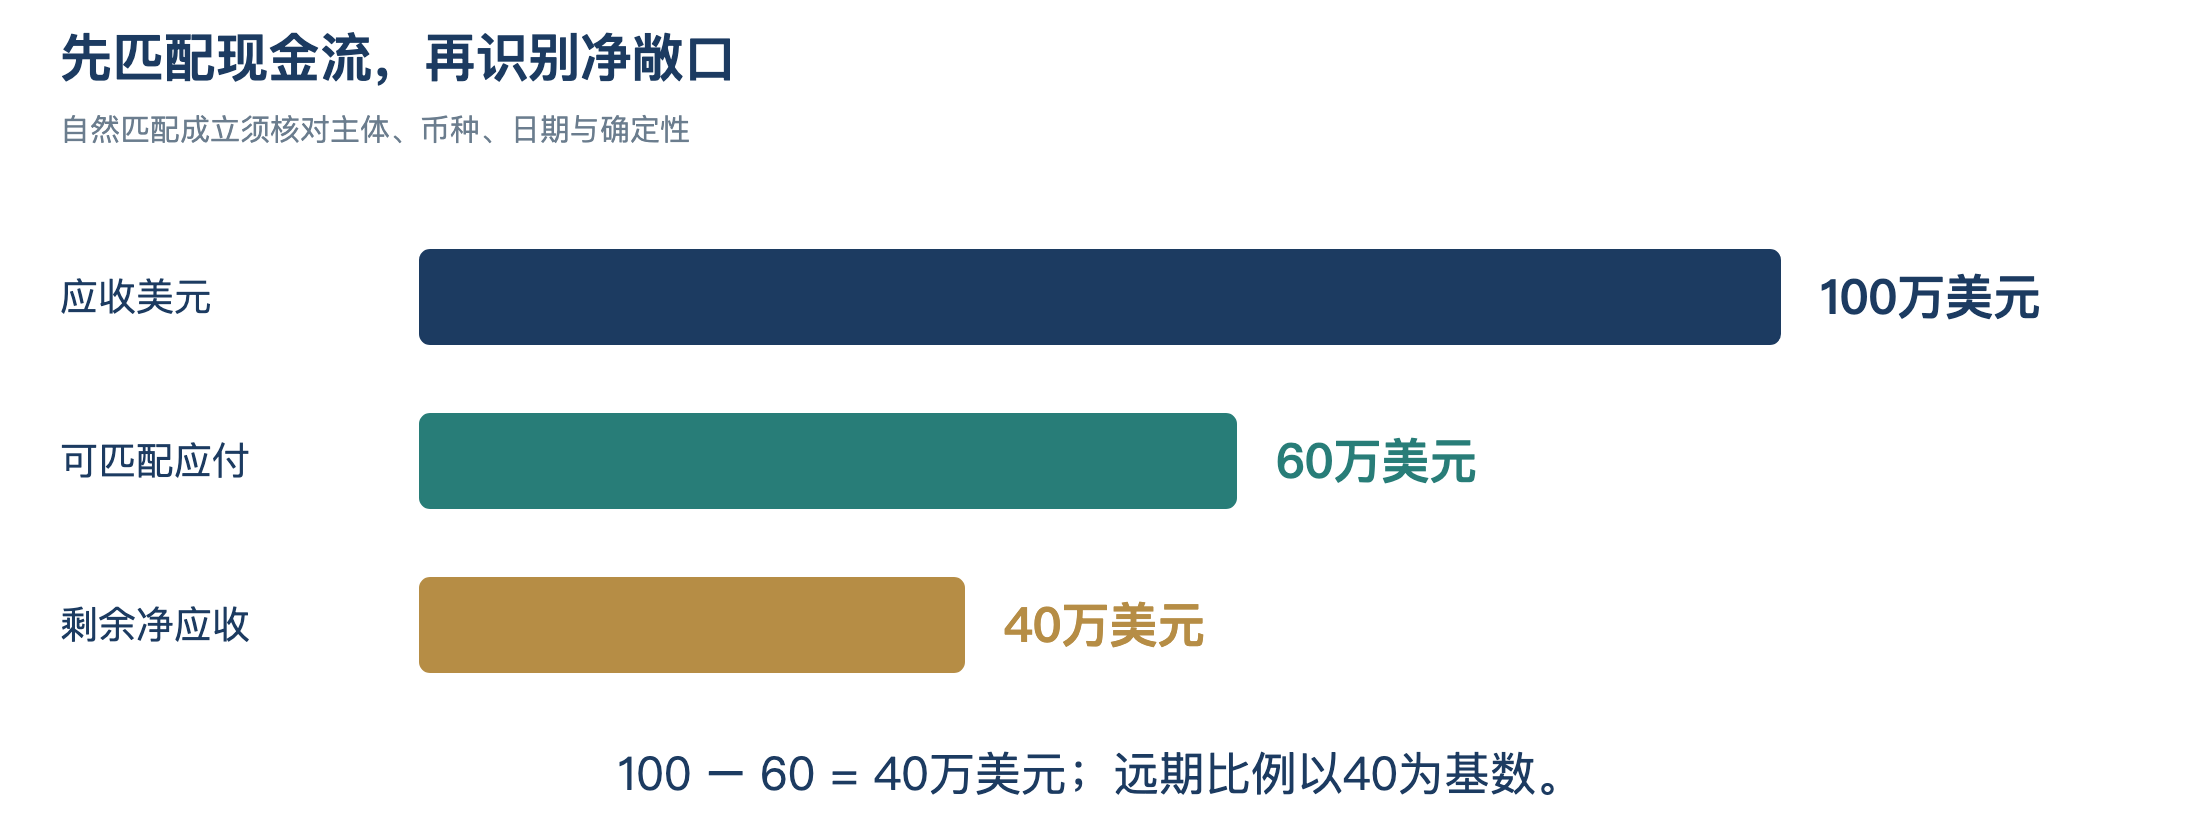
\includegraphics[width=.97\linewidth,height=4.75cm,keepaspectratio,trim=0 0 0 150bp,clip]{figures/03_净敞口.png}\end{center}\[N=100-60=40\quad\text{（万美元，三个月后净应收）}.\]\end{frame}
\renewcommand{\currentweeklabel}{计量}\begin{frame}[t]{不套保：人民币金额如何变化}\relax\hypertarget{slide9}{}\fontsize{10.5}{12.8}\selectfont\setlength{\abovedisplayskip}{.25em}\setlength{\belowdisplayskip}{.25em}\[R_0(e)=Ne=40e\quad\text{（万元人民币）}.\]{\fontsize{9.8}{12}\selectfont\renewcommand{\arraystretch}{1.28}\begin{tabularx}{\linewidth}{@{}>{\raggedright\arraybackslash}X>{\raggedright\arraybackslash}X>{\raggedright\arraybackslash}X@{}}\toprule \textbf{到期汇率\(e\)} & \textbf{代入计算} & \textbf{净收入}\\\midrule 6.80 & \(40\times 6.80\) & 272万元\\
7.10 & \(40\times 7.10\) & 284万元\\
7.40 & \(40\times 7.40\) & 296万元\\\bottomrule\end{tabularx}}\begin{exampleblock}{计量边界}三个汇率是情景设定，不是预测，也没有附加概率。\end{exampleblock}\end{frame}
\renewcommand{\currentweeklabel}{对冲}\begin{frame}[t]{自然对冲：先用经营现金流匹配}\relax\hypertarget{slide10}{}\fontsize{10.5}{12.8}\selectfont\setlength{\abovedisplayskip}{.25em}\setlength{\belowdisplayskip}{.25em}\begin{columns}[T,onlytextwidth]\begin{column}{.48\textwidth}\begin{itemize}\setlength{\itemsep}{.45em}\item 应收100万美元中的60万美元用于同日应付。
\item 剩余40万美元才是本例需要进一步管理的净应收。
\item 自然对冲减少外汇交易需求，但不能忽略日期、资金可用性和确定性。\end{itemize}\end{column}\begin{column}{.48\textwidth}{\fontsize{9.8}{12}\selectfont\renewcommand{\arraystretch}{1.28}\begin{tabularx}{\linewidth}{@{}>{\raggedright\arraybackslash}X>{\raggedright\arraybackslash}X@{}}\toprule \textbf{现金流安排} & \textbf{美元金额}\\\midrule 到期收入 & ＋100万美元\\
匹配应付 & \(-60\,\text{万美元}\)\\
剩余净应收 & ＋40万美元\\\bottomrule\end{tabularx}}\end{column}\end{columns}\begin{exampleblock}{防止重复套保}自然匹配部分不再按应收总额重复卖出；否则可能形成反向敞口。\end{exampleblock}\end{frame}
\renewcommand{\currentweeklabel}{对冲}\begin{frame}[t]{远期结汇：方向、金额与日期匹配}\relax\hypertarget{slide11}{}\fontsize{10.5}{12.8}\selectfont\setlength{\abovedisplayskip}{.25em}\setlength{\belowdisplayskip}{.25em}\begin{center}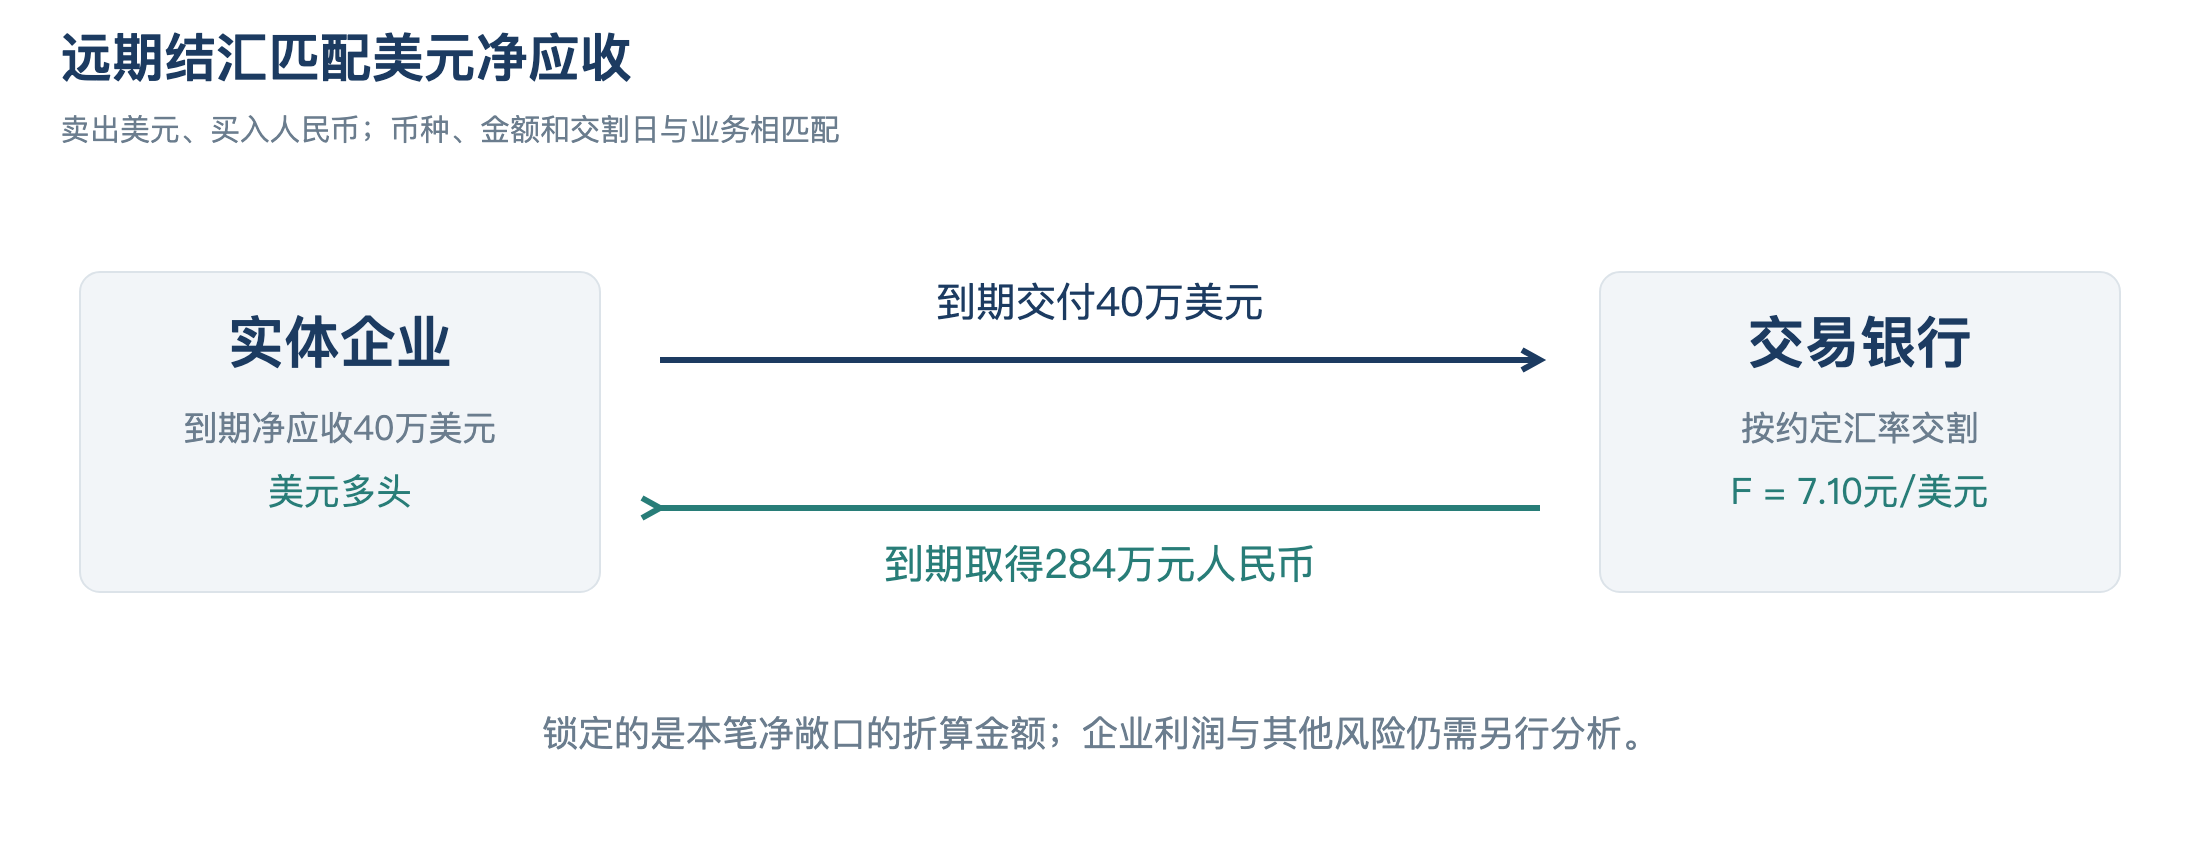
\includegraphics[width=.97\linewidth,height=4.75cm,keepaspectratio,trim=0 0 0 150bp,clip]{figures/04_远期机制.png}\end{center}\begin{exampleblock}{本例100\%套保}对剩余40万美元办理三个月后远期卖出美元，取得284万元人民币。\end{exampleblock}\end{frame}
\renewcommand{\currentweeklabel}{对冲}\begin{frame}[t]{统一表达三种套保比例}\relax\hypertarget{slide12}{}\fontsize{10.5}{12.8}\selectfont\setlength{\abovedisplayskip}{.25em}\setlength{\belowdisplayskip}{.25em}\begin{align*}
R_h(e)&=N\left[hF+(1-h)e\right],\\
N&=40,\quad F=7.10,\quad 0\leq h\leq1,\\
R_{0}(e)&=40e,\\
R_{0.5}(e)&=20\times7.10+20e,\\
R_{1}(e)&=40\times7.10=284.
\end{align*}\begin{exampleblock}{统一口径}金额单位为万元人民币；\(h\)以40万美元净敞口为基数。忽略费用、融资与违约。\end{exampleblock}\end{frame}
\renewcommand{\currentweeklabel}{对冲}\begin{frame}[t]{同口径比较：稳定性与机会收益}\relax\hypertarget{slide13}{}\fontsize{10.5}{12.8}\selectfont\setlength{\abovedisplayskip}{.25em}\setlength{\belowdisplayskip}{.25em}{\fontsize{9.8}{12}\selectfont\renewcommand{\arraystretch}{1.28}\begin{tabularx}{\linewidth}{@{}>{\raggedright\arraybackslash}X>{\raggedright\arraybackslash}X>{\raggedright\arraybackslash}X>{\raggedright\arraybackslash}X@{}}\toprule \textbf{到期汇率} & \textbf{0\%套保} & \textbf{50\%套保} & \textbf{100\%套保}\\\midrule 6.80 & 272 & 278 & 284\\
7.10 & 284 & 284 & 284\\
7.40 & 296 & 290 & 284\\
情景内收入区间 & 272—296 & 278—290 & 284—284\\\bottomrule\end{tabularx}}\begin{exampleblock}{读表结论}比例越高，本笔折算收入对汇率越不敏感；但有利汇率变化带来的机会收益也相应减少。\end{exampleblock}\end{frame}
\renewcommand{\currentweeklabel}{对冲}\begin{frame}[t]{用曲线观察残余敞口}\relax\hypertarget{slide14}{}\fontsize{10.5}{12.8}\selectfont\setlength{\abovedisplayskip}{.25em}\setlength{\belowdisplayskip}{.25em}\begin{center}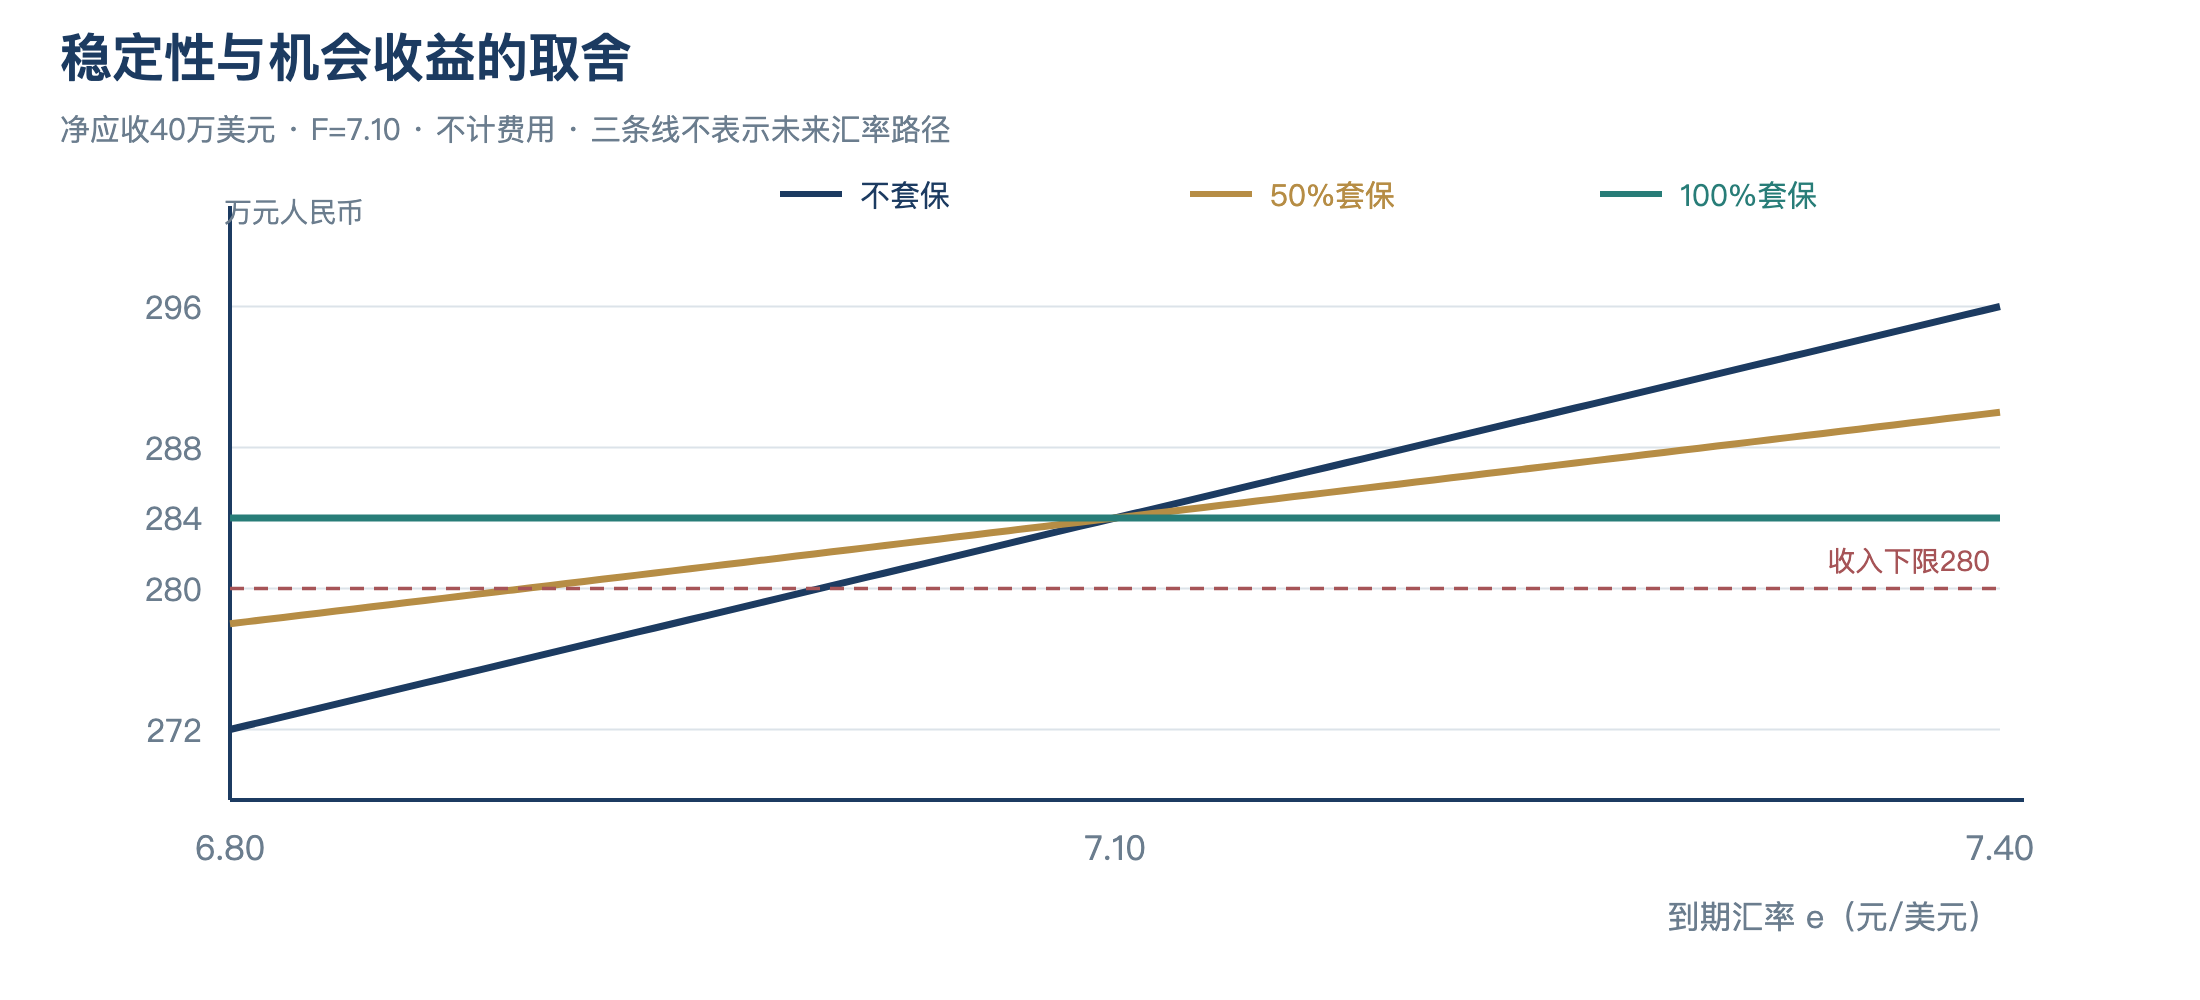
\includegraphics[width=.97\linewidth,height=5.5cm,keepaspectratio,trim=0 0 0 150bp,clip]{figures/05_收入情景曲线.png}\end{center}{\fontsize{9}{11}\selectfont 0\%、50\%、100\%套保对应敏感金额4、2、0万元/每0.10元汇率变化。\par}\end{frame}
\renewcommand{\currentweeklabel}{对冲}\begin{frame}[t]{第一学时归纳：先匹配，再管理}\relax\hypertarget{slide15}{}\fontsize{10.5}{12.8}\selectfont\setlength{\abovedisplayskip}{.25em}\setlength{\belowdisplayskip}{.25em}\begin{itemize}\setlength{\itemsep}{.45em}\item 风险对象：已确定的美元净应收，首先是交易风险。
\item 净敞口：\(100-60=40\,\text{万美元}\)，日期为三个月后。
\item 交易安排：净应收对应远期卖出美元；比例以净额为基数。\end{itemize}\begin{exampleblock}{课堂检验}使用独立单选题课件Q3、Q4；先个人作答，再核对净额与交易方向。\end{exampleblock}\end{frame}
\renewcommand{\currentweeklabel}{决策}\begin{frame}[t]{AI赋能：构建可以审查的证据链}\relax\hypertarget{slide16}{}\fontsize{10.5}{12.8}\selectfont\setlength{\abovedisplayskip}{.25em}\setlength{\belowdisplayskip}{.25em}\begin{center}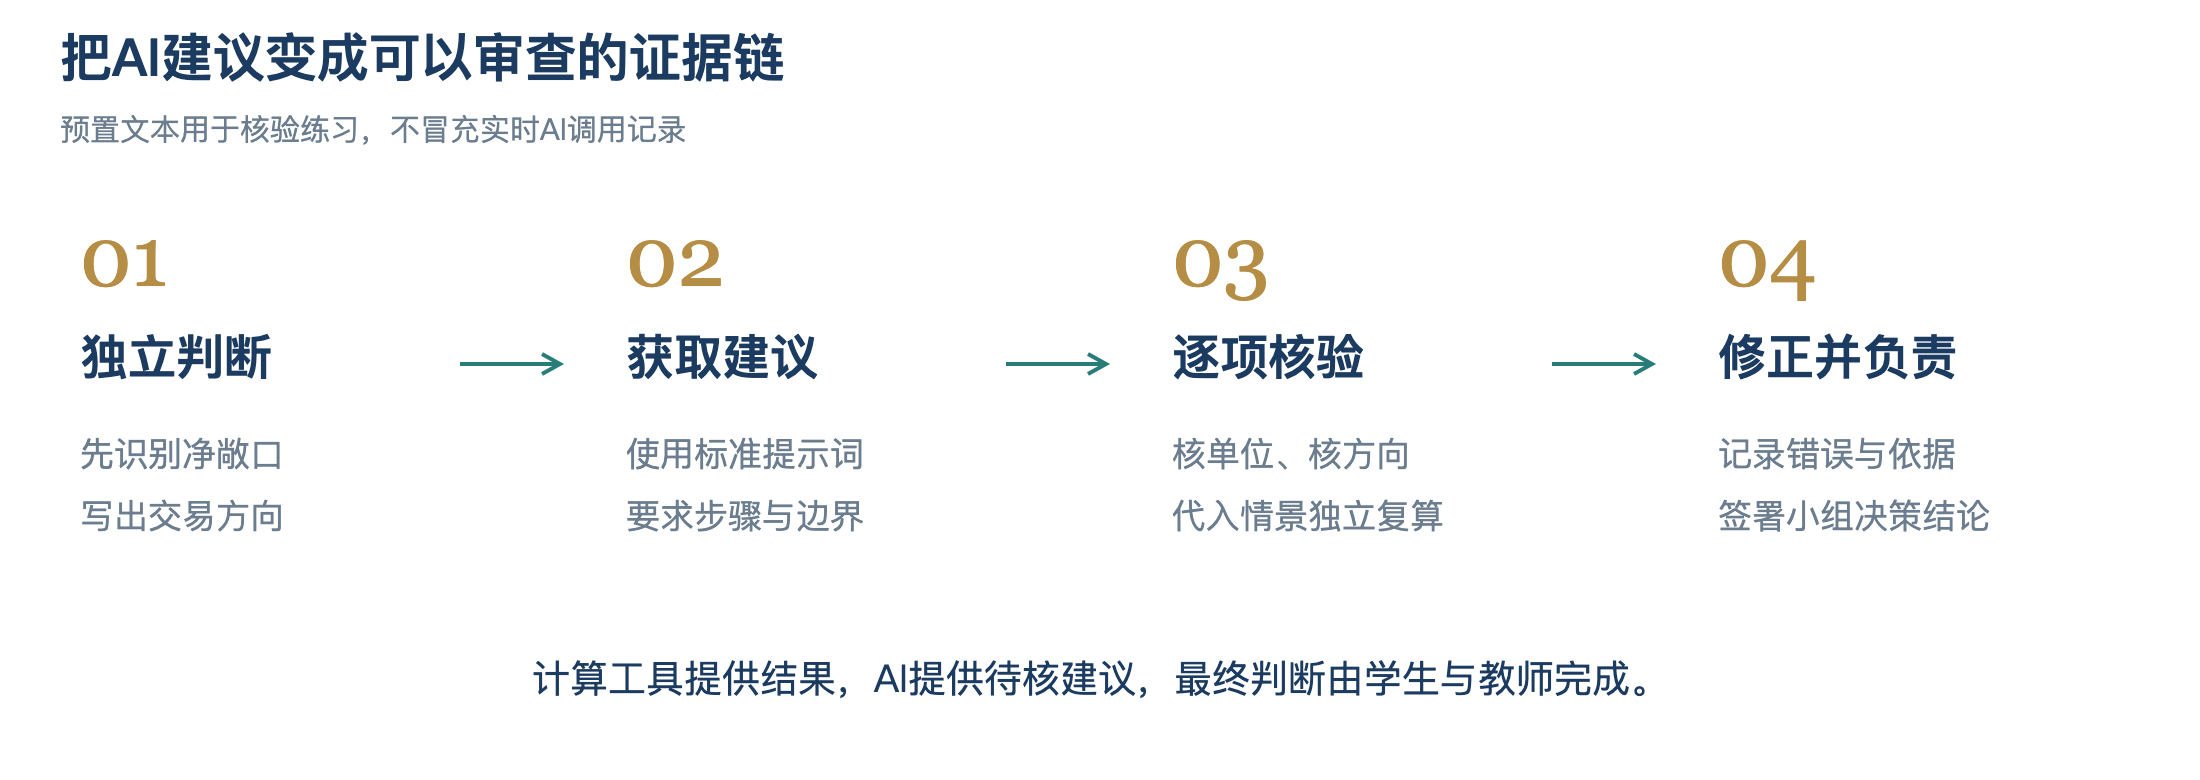
\includegraphics[width=.97\linewidth,height=4.75cm,keepaspectratio,trim=0 0 0 150bp,clip]{figures/06_AI核验路径.png}\end{center}\begin{exampleblock}{12分钟活动}个人复核3分钟，同伴核对5分钟，教师归纳4分钟；记录错误、证据和修正。\end{exampleblock}\note{发放AI核验单；预置文本明确为核验练习，不冒充实时输出。}\end{frame}
\renewcommand{\currentweeklabel}{决策}\begin{frame}[t]{AI核验后的四条专业结论}\relax\hypertarget{slide17}{}\fontsize{10.5}{12.8}\selectfont\setlength{\abovedisplayskip}{.25em}\setlength{\belowdisplayskip}{.25em}{\fontsize{9.8}{12}\selectfont\renewcommand{\arraystretch}{1.28}\begin{tabularx}{\linewidth}{@{}>{\raggedright\arraybackslash}X>{\raggedright\arraybackslash}X@{}}\toprule \textbf{核验焦点} & \textbf{专业结论}\\\midrule 基数 & 先自然匹配，净应收为40万美元\\
方向 & 净应收需要卖出美元；买入会扩大美元多头\\
依据 & 情景不是预测，预算结论须由计算支持\\
边界 & 锁定本笔折算金额，不保证企业利润最高或风险清零\\\bottomrule\end{tabularx}}\begin{exampleblock}{责任归属}HTML是确定性计算工具，AI输出是待核建议，最终判断由学生与教师完成。\end{exampleblock}\note{本页用于核验后讲评，先让学生完成个人记录。}\end{frame}
\renewcommand{\currentweeklabel}{决策}\begin{frame}[t]{预算约束下形成可复核的建议}\relax\hypertarget{slide18}{}\fontsize{10.5}{12.8}\selectfont\setlength{\abovedisplayskip}{.25em}\setlength{\belowdisplayskip}{.25em}\begin{columns}[T,onlytextwidth]\begin{column}{.48\textwidth}\begin{exampleblock}{管理目标}在给定三个情景下，人民币净收入不低于280万元。\end{exampleblock}\end{column}\begin{column}{.48\textwidth}\begin{itemize}\setlength{\itemsep}{.45em}\item 比较0\%、50\%、100\%三种方案。
\item 列出不采纳方案及预算依据。
\item 写清方向、金额、日期与复核条件。\end{itemize}\end{column}\end{columns}{\fontsize{9.8}{12}\selectfont\renewcommand{\arraystretch}{1.28}\begin{tabularx}{\linewidth}{@{}>{\raggedright\arraybackslash}X>{\raggedright\arraybackslash}X>{\raggedright\arraybackslash}X@{}}\toprule \textbf{方案} & \textbf{给定情景内最低收入} & \textbf{达到下限}\\\midrule 0\%套保 & 272万元 & 否\\
50\%套保 & 278万元 & 否\\
100\%套保 & 284万元 & 是\\\bottomrule\end{tabularx}}\note{小组15分钟，使用HTML与决策单；不以预测代替预算。}\end{frame}
\renewcommand{\currentweeklabel}{决策}\begin{frame}[t]{提高任务：区间内的比例下限}\relax\hypertarget{slide19}{}\fontsize{10.5}{12.8}\selectfont\setlength{\abovedisplayskip}{.25em}\setlength{\belowdisplayskip}{.25em}\begin{center}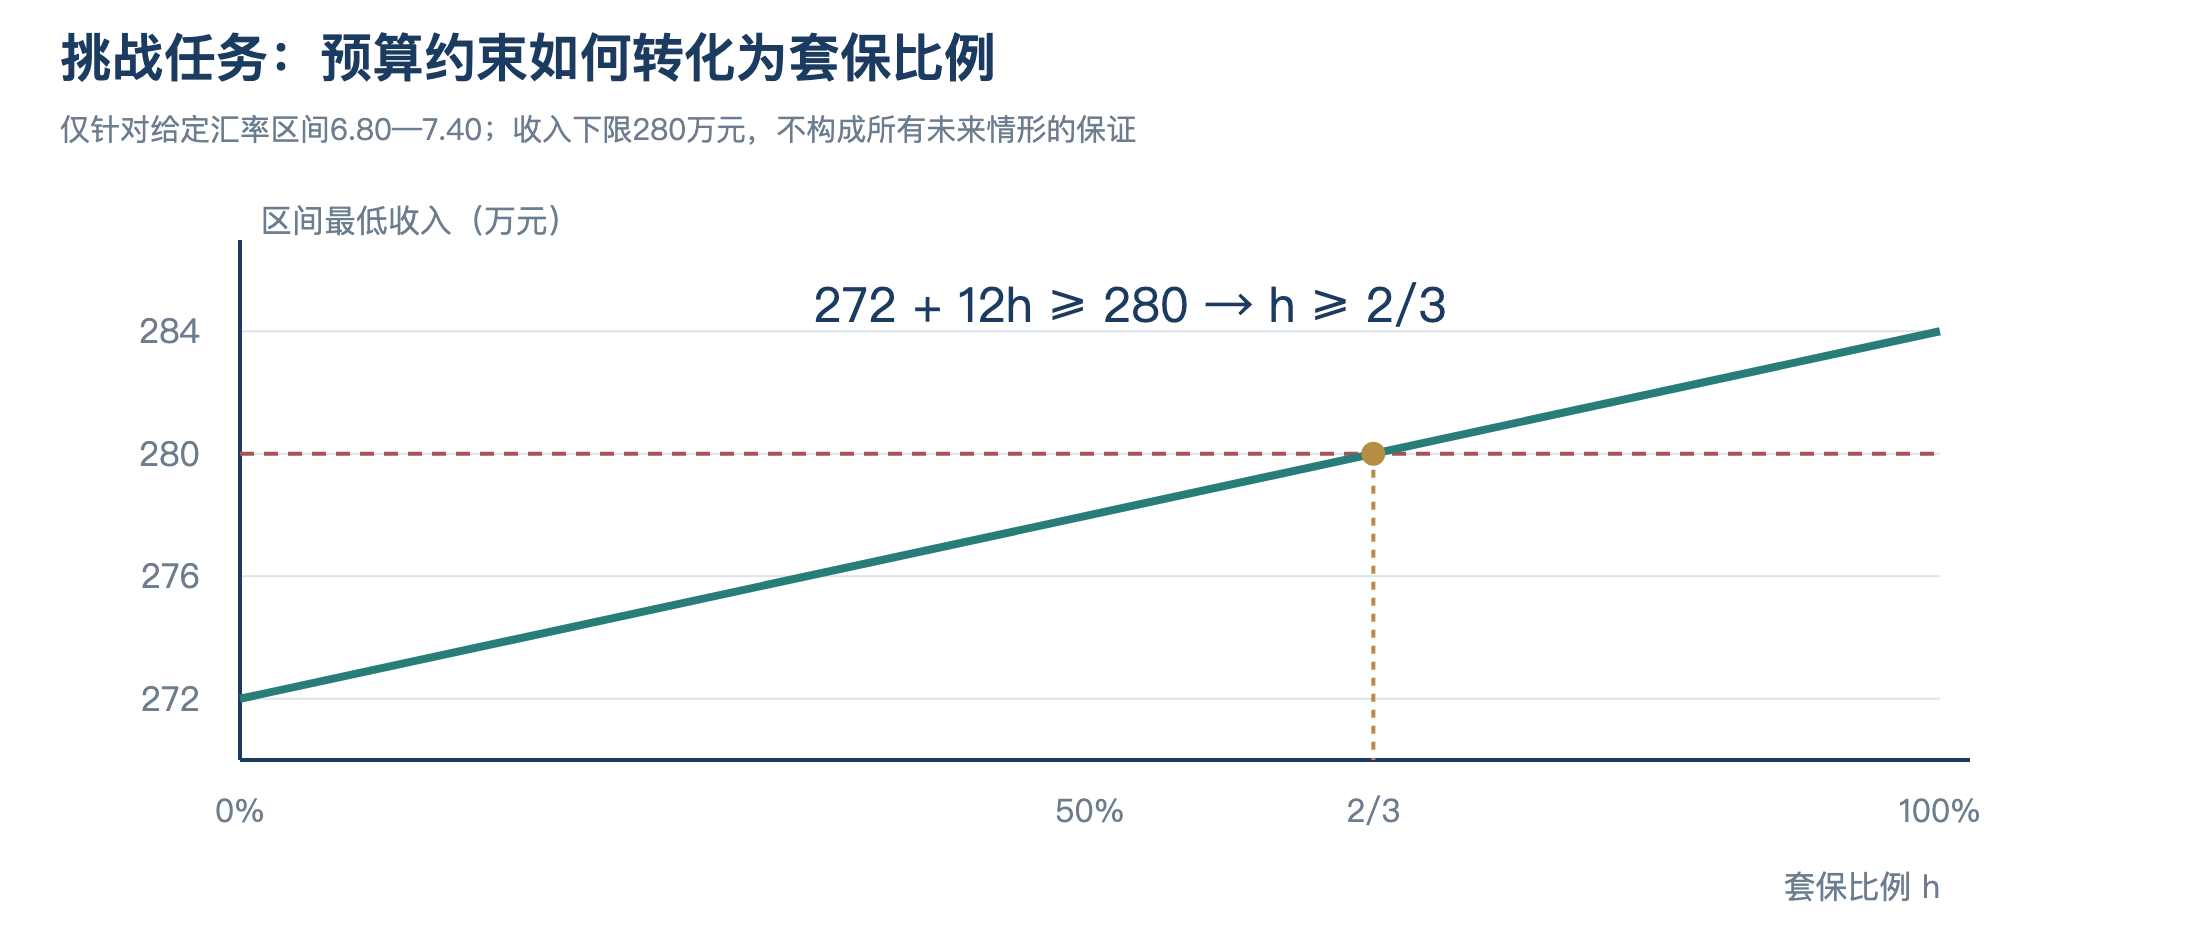
\includegraphics[width=.97\linewidth,height=4.5cm,keepaspectratio,trim=0 0 0 150bp,clip]{figures/08_预算约束.png}\end{center}\[\min_{e\in[6.80,7.40]}R_h(e)=272+12h\geq280\quad\Rightarrow\quad h\geq\frac23.\]\note{可选提高任务；核心班级先完成三个离散方案。不得把区间结果扩大为任意未来汇率保证。}\end{frame}
\renewcommand{\currentweeklabel}{决策}\begin{frame}[t]{条件改变：日期错配必须重新评估}\relax\hypertarget{slide20}{}\fontsize{10.5}{12.8}\selectfont\setlength{\abovedisplayskip}{.25em}\setlength{\belowdisplayskip}{.25em}\begin{center}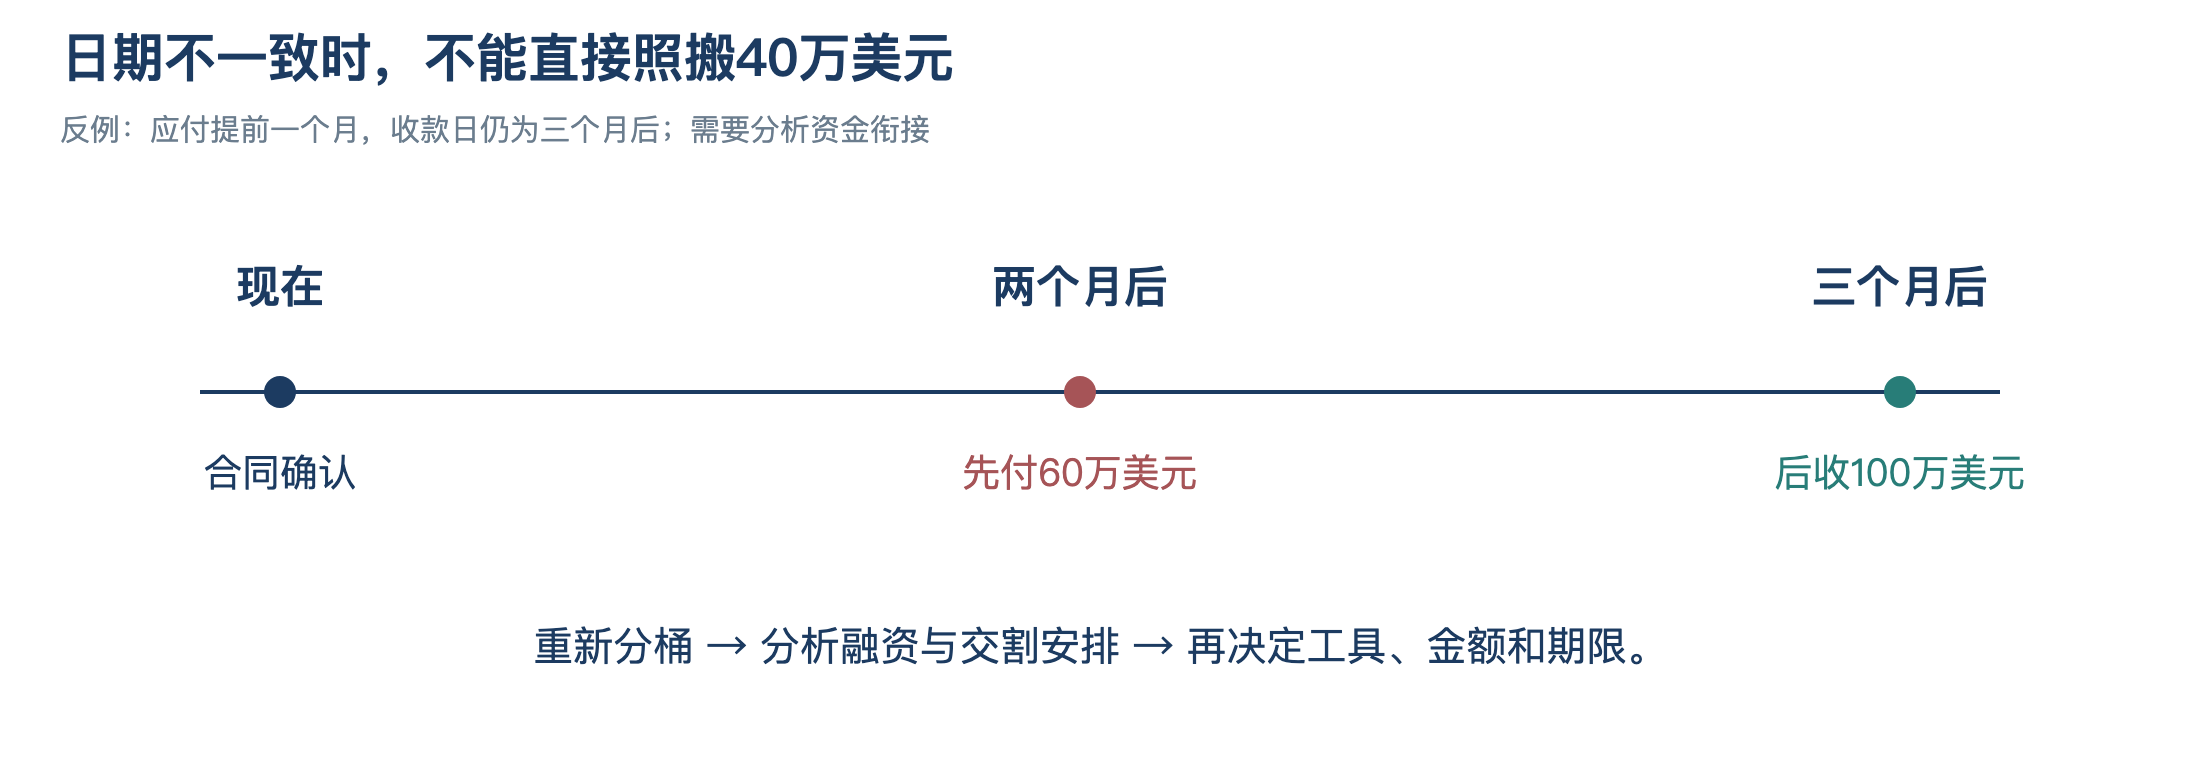
\includegraphics[width=.97\linewidth,height=4.75cm,keepaspectratio,trim=0 0 0 150bp,clip]{figures/09_日期错配.png}\end{center}\begin{exampleblock}{复核触发}收付日期、订单规模、币种、确定性或资金可用性变化时，重新分桶并评估工具。\end{exampleblock}\note{供小组讨论的边界提示，不要求计算复杂融资或掉期定价。}\end{frame}
\renewcommand{\currentweeklabel}{决策}\begin{frame}[t]{展示与点评：看结论背后的证据}\relax\hypertarget{slide21}{}\fontsize{10.5}{12.8}\selectfont\setlength{\abovedisplayskip}{.25em}\setlength{\belowdisplayskip}{.25em}{\fontsize{9.8}{12}\selectfont\renewcommand{\arraystretch}{1.28}\begin{tabularx}{\linewidth}{@{}>{\raggedright\arraybackslash}X>{\raggedright\arraybackslash}X>{\raggedright\arraybackslash}X@{}}\toprule \textbf{评价维度} & \textbf{得分} & \textbf{充分达成的表现}\\\midrule 专业正确 & 12 & 净额、方向、金额、日期、单位与公式一致\\
证据与推理 & 9 & 情景表完整，预算结论可复算\\
风险边界 & 6 & 说明假设、不能保证的结果及复核条件\\
表达 & 3 & 结论简洁，图表与依据相互对应\\\bottomrule\end{tabularx}}\begin{exampleblock}{时间安排}两组各3分钟，教师综合点评4分钟；其余小组提交书面决策单。\end{exampleblock}\end{frame}
\renewcommand{\currentweeklabel}{决策}\begin{frame}[t]{价值引领体现在负责任的专业行动中}\relax\hypertarget{slide22}{}\fontsize{10.5}{12.8}\selectfont\setlength{\abovedisplayskip}{.25em}\setlength{\belowdisplayskip}{.25em}{\fontsize{9.8}{12}\selectfont\renewcommand{\arraystretch}{1.28}\begin{tabularx}{\linewidth}{@{}>{\raggedright\arraybackslash}X>{\raggedright\arraybackslash}X@{}}\toprule \textbf{行动} & \textbf{可观察的学习证据}\\\midrule 服务实体经营 & 从订单履约、预算与风险承受能力界定目标\\
诚信与敬业 & 不隐藏不利情景，不编造资料或AI运行记录\\
审慎与责任 & 报告假设和风险边界，说明何时需要重新评估\\
交叉融合 & 结合经济分析、财务计算与数字工具核验结论\\\bottomrule\end{tabularx}}\begin{exampleblock}{专业评价原则}按可观察的专业表现评价，不以口号数量代替知识与能力。\end{exampleblock}\end{frame}
\renewcommand{\currentweeklabel}{归纳}\begin{frame}[t]{迁移：美元净应付改变交易方向}\relax\hypertarget{slide23}{}\fontsize{10.5}{12.8}\selectfont\setlength{\abovedisplayskip}{.25em}\setlength{\belowdisplayskip}{.25em}\begin{center}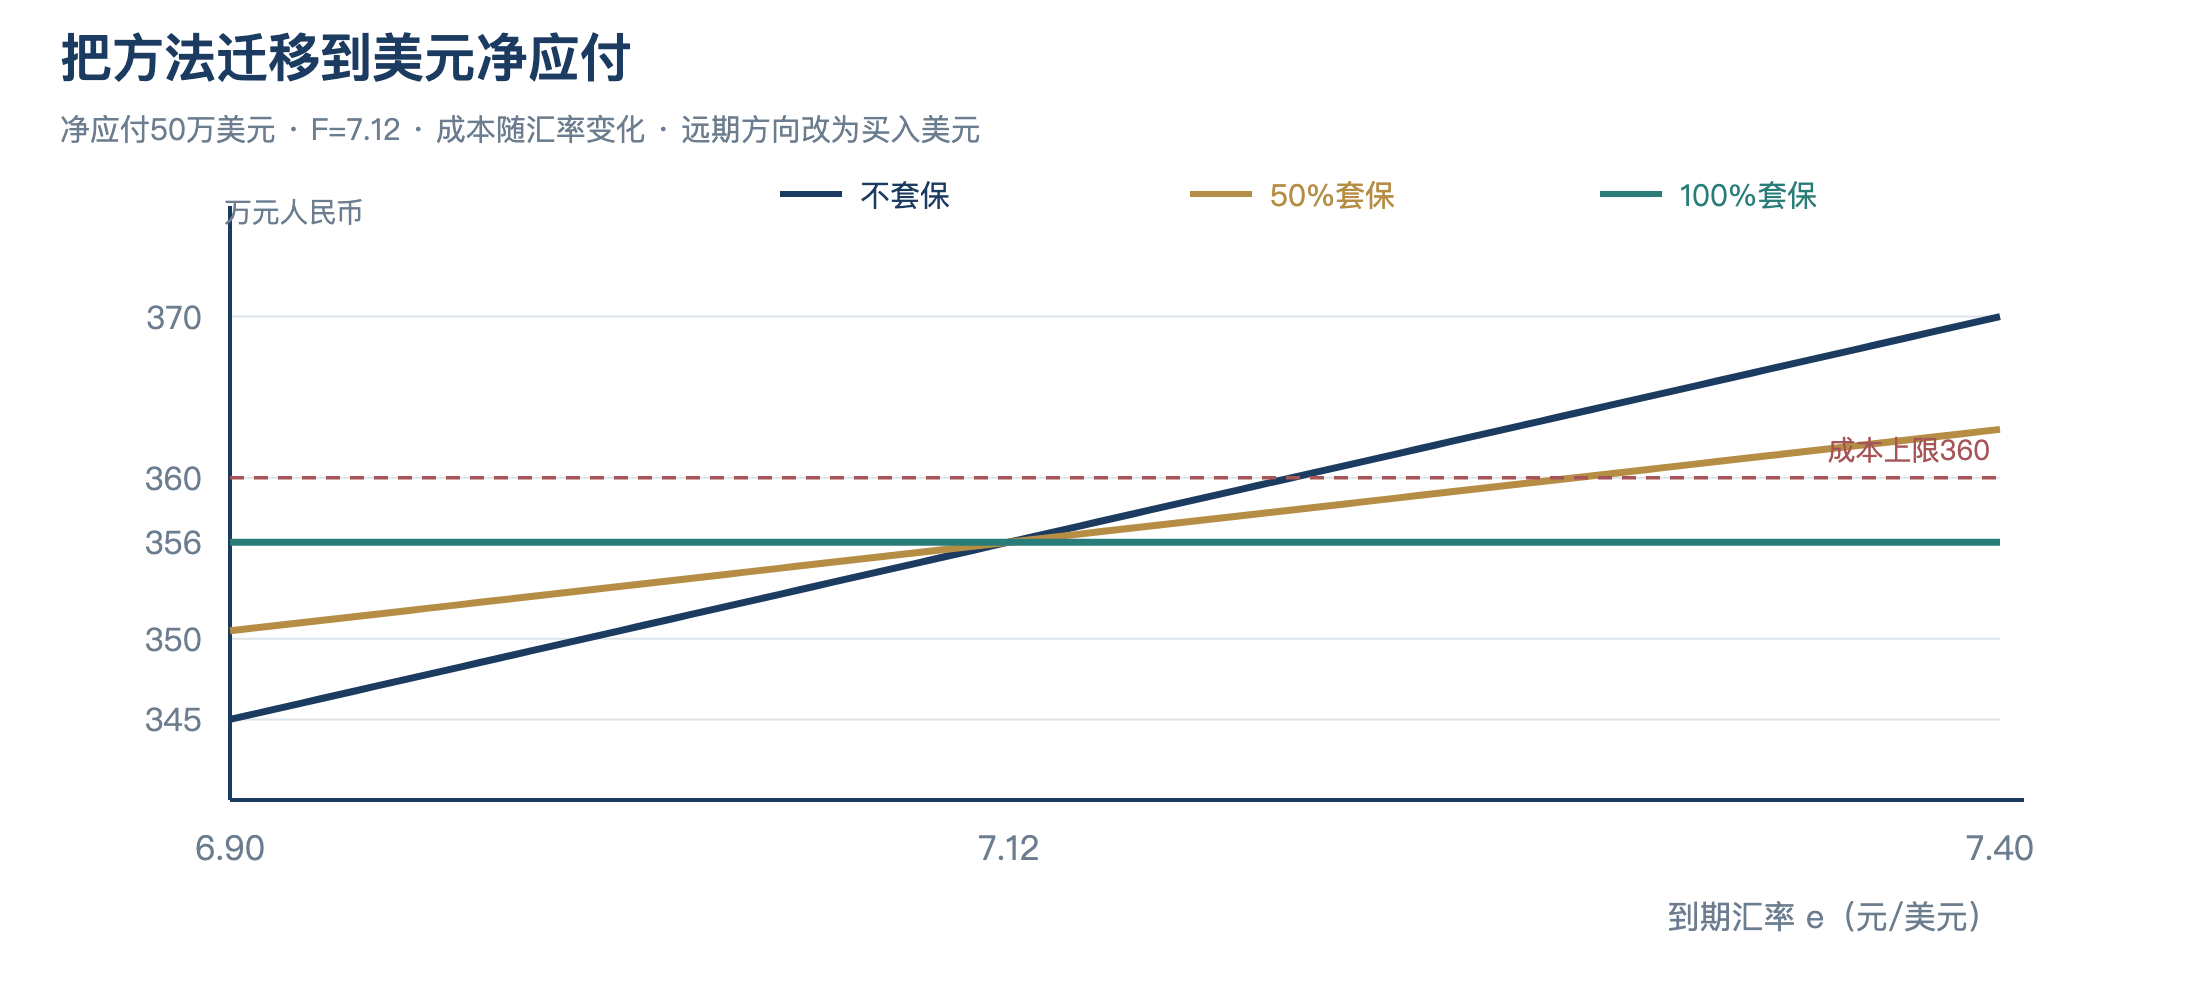
\includegraphics[width=.97\linewidth,height=4.35cm,keepaspectratio,trim=0 0 0 150bp,clip]{figures/11_进口迁移曲线.png}\end{center}\begin{exampleblock}{课后任务}同日付80万、收30万美元，远期购汇7.12；比较三个方案能否在给定情景下将净付款成本控制在360万元以内。\end{exampleblock}\note{展示任务与方法，完整参考答案见教师附件；不提前替学生完成课后分析。}\end{frame}
\renewcommand{\currentweeklabel}{归纳}\begin{frame}[t]{把方法迁移到下一笔业务}\relax\hypertarget{slide24}{}\fontsize{10.5}{12.8}\selectfont\setlength{\abovedisplayskip}{.25em}\setlength{\belowdisplayskip}{.25em}\begin{center}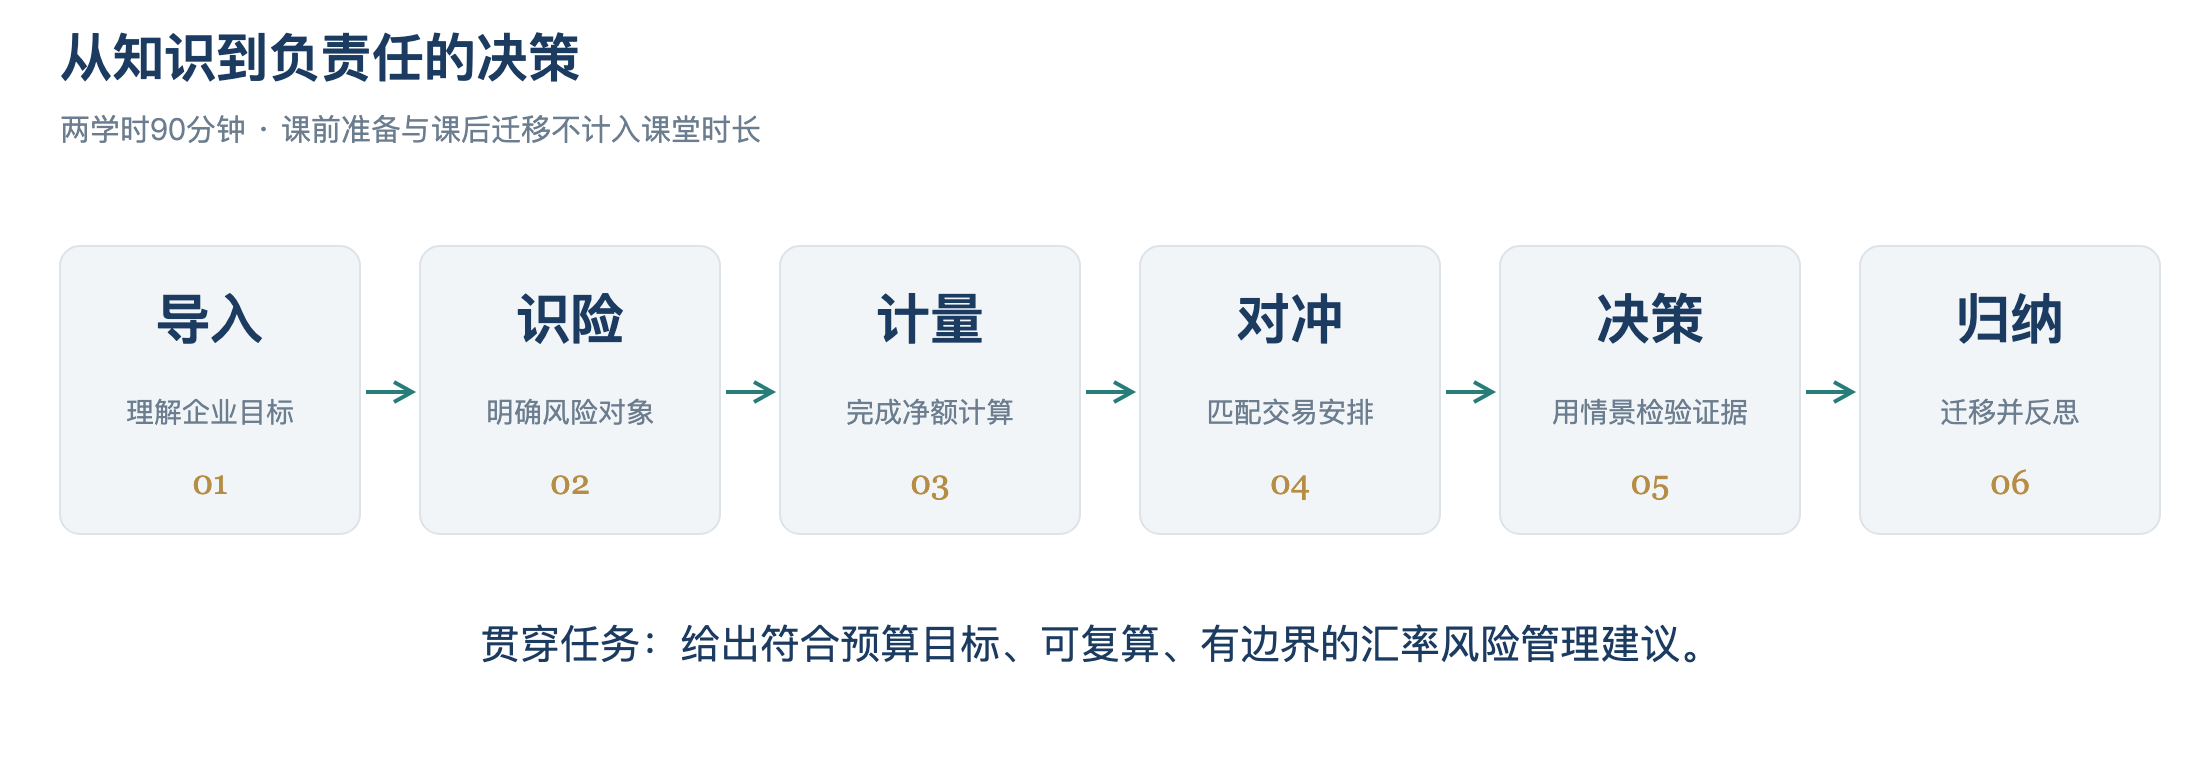
\includegraphics[width=.97\linewidth,height=4.1cm,keepaspectratio,trim=0 0 0 150bp,clip]{figures/07_教学路径.png}\end{center}\begin{itemize}\setlength{\itemsep}{.45em}\item 先核对事实，再计算净敞口；先确定目标，再选择管理安排。
\item 用情景与独立计算核验建议，以经营变化触发复核。\end{itemize}\end{frame}
\renewcommand{\currentweeklabel}{归纳}\begin{frame}[t]{保留学习证据，形成持续改进}\relax\hypertarget{slide25}{}\fontsize{10.5}{12.8}\selectfont\setlength{\abovedisplayskip}{.25em}\setlength{\belowdisplayskip}{.25em}\begin{center}
\includegraphics[width=.97\linewidth,height=4cm,keepaspectratio,trim=0 0 0 150bp,clip]{figures/10_目标评价.png}\end{center}\begin{exampleblock}{本讲评价}课前10、课堂20、AI核验20、小组30、课后20；课末完成独立题目课件Q5、Q6。\end{exampleblock}\note{本页可备查。收集真实成绩与匿名反馈后再记录反思，不预写成效。}\end{frame}
\renewcommand{\currentweeklabel}{归纳}\begin{frame}[t]{教材与专业核验依据}\relax\hypertarget{slide26}{}\fontsize{10.5}{12.8}\selectfont\setlength{\abovedisplayskip}{.25em}\setlength{\belowdisplayskip}{.25em}\begin{itemize}\setlength{\itemsep}{.45em}\item 教材：范小云、陈平主编《国际金融》第二版，第九章第一节，第256—266页。
\item 回信：2026年9月28日习近平总书记给四川大学全体师生的回信，教育部网站刊载。
\item 国家外汇管理局《企业汇率风险管理指引（2024年版）》及四川省分局风险中性公开材料。
\item 案例金额为设定；图表原创。假设、出处与详细网址见教案第12页及HTML资料区。\end{itemize}\begin{exampleblock}{边界说明}本讲不预测未来汇率，不包含期权定价、复杂套保会计或真实企业业绩数据。\end{exampleblock}\end{frame}
\end{document}